\input{../templates/course_definitions}
% This Document contains the information about this course.

% Authors of the slides
\author{Tobias Hanf, Manik Khurana}

% Name of the Course
\institute{Java-Course}

% Fancy Logo
\titlegraphic{\hfill\includegraphics[height=1.25cm]{../templates/fsr_logo_cropped}}


\title{Java}
\subtitle{Sets & Maps}
\date{\today}

\begin{document}
	
	\begin{frame}
		\titlepage
	\end{frame}
	
	\begin{frame}{Overview}
		\tableofcontents
	\end{frame}
	
	\section{Recap}
	\subsection{Last class' exercise - Collections}
	\begin{frame}{Last class' exercise - Collections}
		"This class consists exclusively of static methods that operate on or return collections"\footnote{\url{https://docs.oracle.com/en/java/javase/11/docs/api/java.base/java/util/Collections.html}}
		
		Some methods:
		\begin{itemize}
			\item \texttt{binarySearch(...)}
			\item \texttt{max(...)}
			\item \texttt{min(...)}
			\item \texttt{reverse(...)}
			\item \texttt{sort(...)}
		\end{itemize}
	\end{frame}
\subsection {Hands-on Exercise}
	\begin{frame}{Part 3 - Contd. from last class}
		
		\begin{center}
			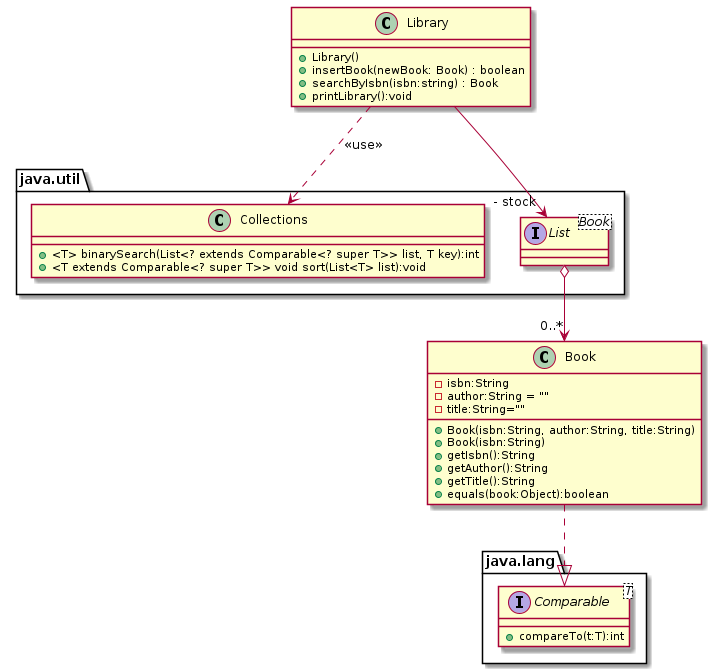
\includegraphics[scale=.34]{07_collection/hands_on_03.png}
		\end{center}
		
	\end{frame}
	
	\begin{frame}{Part 4- Contd. from last class}
		
		\begin{center}
			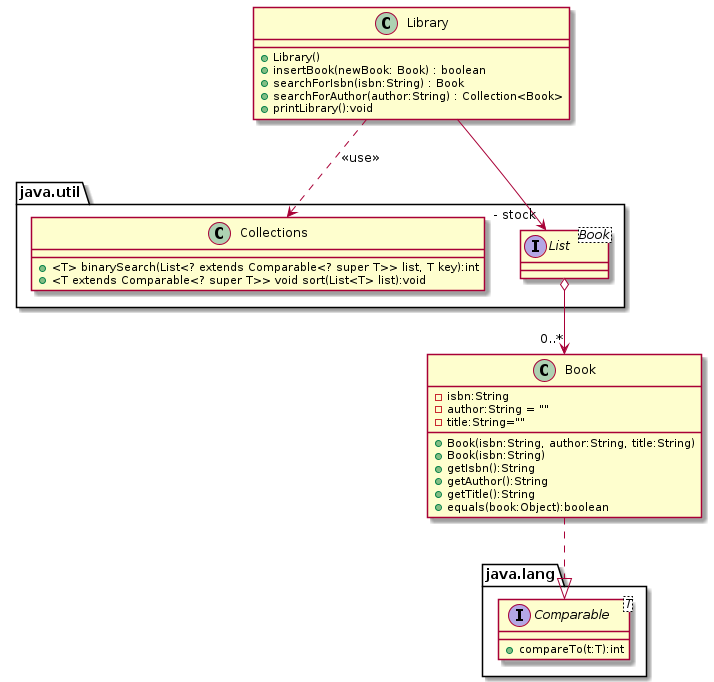
\includegraphics[scale=.34]{07_collection/hands_on_04.png}
		\end{center}
		
	\end{frame}	
	
	
	\section{Set}
	
	\begin{frame}{Collections Framework}
		Java offers various data structures like \textbf{Sets}, \textbf{Lists} and \textbf{Maps}.
		Those structures are part of the collections framework.
		
		There are interfaces to access the data structures in an easy way.
		There are multiple implementations for various needs.
		Alternatively you can use your own implementations.
		
		Documentation: \url{https://docs.oracle.com/en/java/javase/11/docs/api/java.base/java/util/Collection.html}
	\end{frame}
	
	\begin{frame}{Collections Overview}
		
		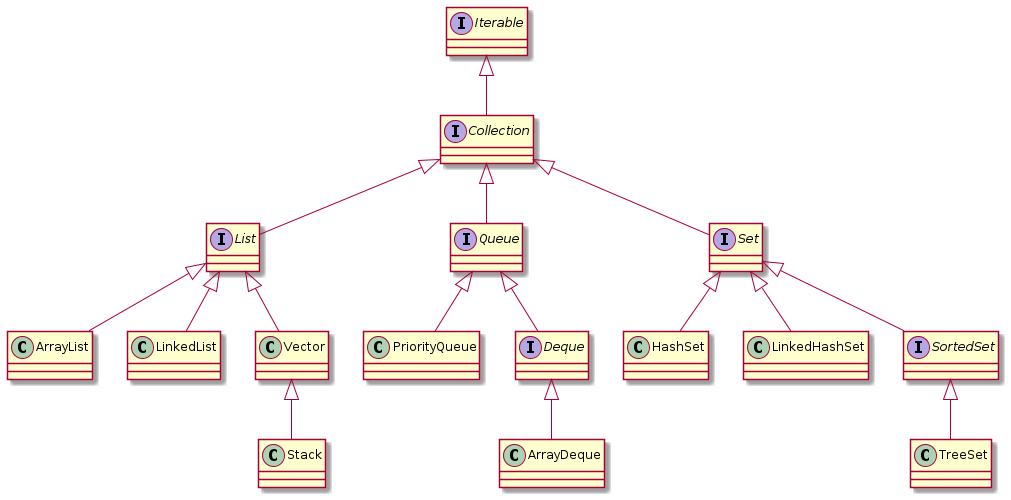
\includegraphics[width=\textwidth]{07_collection/collection.png}
	\end{frame}
	
	\begin{frame}[fragile]{Set}
		The set interface is present in java.util package and extends the Collection interface is an unordered collection of objects in which duplicate values cannot be stored. 
		
		The Set interface is declared as:
		\begin{lstlisting}
			public interface Set extends Collection 
		\end{lstlisting}
		
		The Set object can be created as:
		\begin{lstlisting}
			// Obj is the type of the object to be stored in Set 
			Set<Obj> set = new HashSet<Obj> (); 
		\end{lstlisting}
		
	\end{frame}
	
	\begin{frame}[fragile]{Set Methods}
		some useful Set methods:\\
		\vspace{1em}
		\begin{tabular}{ r l r }
			boolean & \texttt{add(E element)}
			& \footnotesize{insert element if not already present} \\
			boolean &\texttt{contains(Object o)}
			& \footnotesize{Returns true if the specified element is present} \\
			int &\texttt{size()}
			& \footnotesize{Returns the number of elements in the set} \\
		\end{tabular}
	
	\end{frame}
	
\section{Map}
	\begin{frame}
		\begin{center}
			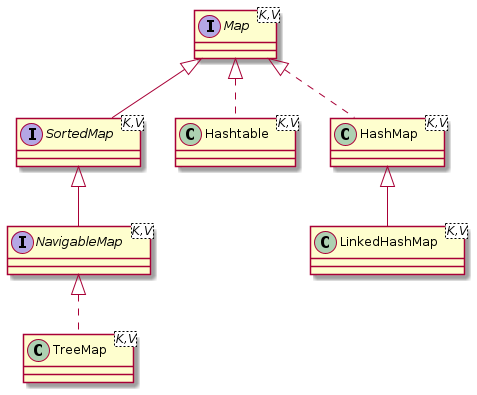
\includegraphics[scale=.5]{08_set_map/maps.png}
		\end{center}
		
	\end{frame}

	\begin{frame}[fragile]{Map}
		The interface \emph{Map} is not a subinterface of \emph{Collection}.\\
		A map contains pairs of key and value. Each key refers to a value. 
		Two keys can refer to the same value. There are not two equal keys in one map.
		\emph{Map} is part of the package \texttt{java.util}.
		\vfill
		\begin{lstlisting}[basicstyle=\ttfamily\scriptsize]
			public static void main (String[] args) {
				
				Map<Integer, String> map = 
				new HashMap<Integer, String>();
				
				map.put(23, "foo");
				map.put(28, "foo");
				map.put(31, "bar");
				map.put(23, "bar"); // "bar" replaces "foo" for key = 23
				
				System.out.println(map);
				// prints: {23=bar, 28=foo, 31=bar}
			}
		\end{lstlisting}
	\end{frame}
	
	\begin{frame}[fragile]{Key, Set and Values}
		You can get the set of keys from the map.
		Because one value can exist multiple times a collection is used for the values.
		\begin{lstlisting}[basicstyle=\ttfamily\scriptsize]
			public static void main (String[] args) {
				
				// [...] map like previous slide
				
				Set<Integer> keys = map.keySet();
				Collection<String> values = map.values();
				
				System.out.println(keys);
				// prints: [23, 28, 31]
				
				System.out.println(values);
				// prints: [bar, foo, bar]
			}
		\end{lstlisting}
	\end{frame}
	
	
	\begin{frame}[fragile]{Nested Maps}
		Nested maps offer storage with key pairs.
		\begin{lstlisting}[basicstyle=\ttfamily\scriptsize]
			public static void main (String[] args) {		
				
				Map<String, Map<Integer, String>> addresses = 
				new HashMap<String, Map<Integer, String>>();
				
				addresses.put("Noethnitzer Str.", 
				new HashMap<Integer, String>());
				
				addresses.get("Noethnitzer Str.").
				put(46, "Andreas-Pfitzmann-Bau");
				addresses.get("Noethnitzer Str.").
				put(44, "Fraunhofer IWU");
			}
		\end{lstlisting}
	\end{frame}
	
	\begin{frame}[fragile]{Maps and Lambda}
		\begin{lstlisting}[basicstyle=\ttfamily\scriptsize]
			map.forEach((k,v) -> {
				//Key and Value
				System.out.println("Key: " + k + ", value: " v);
			})
		\end{lstlisting}
	\end{frame}
	
	\begin{frame}[fragile]{Maps and For Each}
		You can interate through the entry set of a map (available before Java 1.8)
		\begin{lstlisting}[basicstyle=\ttfamily\scriptsize]
			Map<String, String> map = ...
			for (Map.Entry<String, String> entry : map.entrySet()) {
				System.out.println("Key: " + entry.getKey() +
				", value" + entry.getValue());
			}
		\end{lstlisting}
	\end{frame}
	
		\begin{frame}[fragile]{Map Methods}
		some useful Map methods:\\
		\vspace{1em}
		\begin{tabular}{ r l l }
			\texttt{V} & \texttt{get(Object key)}
			& \\
			& \footnotesize{Returns the value to which the specified key is mapped.} \\
			\texttt{V} & \texttt{remove(Object key)}
			& \\
			& \footnotesize{Removes the mapping for a key from this map if it is present} \\
			\texttt{V} &\texttt{put(K key, V value)}
			& \\
			& \footnotesize{Associates the specified value with the specified key in this map} \\
			\texttt{Collection<V>} &\texttt{values()}
			& \\
			& \footnotesize{Returns a collection view of the values contained in the map} \\
			\texttt{Set<K>} &\texttt{keySet()}
			& \\
			& \footnotesize{Returns a set view of the keys contained in the map} \\
		\end{tabular}
		
	\end{frame}
	
	
	\begin{frame}[allowframebreaks]{TreeMap vs HashMap}
		
		TreeMap\footnote{ \url{https://docs.oracle.com/en/java/javase/11/docs/api/java.base/java/util/TreeMap.html}}:
		\begin{itemize}
			\item Red-Black tree implementation
			\item has an ordering $\rightarrow$ can be sorted
			\item guaranteed \texttt{log(n)} time constant for \texttt{get}, \texttt{put} and \texttt{remove}
		\end{itemize}
		
		\framebreak
		HashMap\footnote{\url{https://docs.oracle.com/en/java/javase/11/docs/api/java.base/java/util/HashMap.html}}:
		\begin{itemize}
			\item Hash table implementation
			\item mostly constant time for \texttt{get} and \texttt{put}
			\item \textit{initial capacity} and \textit{load factor} determine performance
		\end{itemize}
		
		
	\end{frame}
	\begin{frame}{Overview}
		\begin{center}
			\begin{tabular}{ l | l }
				List & Keeps order of objects \\
				& Easily traversible \\
				& Search not effective \\
				\hline
				Set  & No duplicates \\
				& No order - still traversible \\
				& Effective searching \\
				\hline
				Map  & Key-Value storage \\
				& Search super-effective \\
				& Traversing difficult
				
			\end{tabular}
		\end{center}
	\end{frame}
	
	
		
\end{document}